\section{Further examples of Simple Harmonic Motion (SHM)} \marginnote[-0.5cm]{\emph{Lecture 2}\\ \noindent Kahoot! Quiz on SHM}
\vspace{-0.5cm}
\newthought{From our basic definition}, we observe SHM when the restoring force is linearly proportional to displacement. \marginnote[0.5cm]{\p{This is because we know that SHM obeys the SHM differential equation!}}
\p{Conversely, if SHM is observed, then we must have
\begin{align}
F_r = -kx \nonumber
\end{align}
} 
Then for any simple harmonic motion we can write out the expression for the \emph{force constant} $k$, 
\begin{align}
k = -\frac{F_x(t)}{x(t)} \qquad \textrm{so that} \qquad \omega = \sqrt{\frac{k}{m}}
\end{align}
where $x(t)$ is measured from the \emph{equilibrium} point. 


\marginnote[5cm]{\p{In general we must have
\begin{align}
\sum F = m a \nonumber
\end{align}
while at the equilibrium point we have
\begin{align}
\sum F = 0.\nonumber
\end{align}
}}
\begin{examplebox}{An Object on a Vertical Spring}
Consider a mass hanging on a vertical spring:

\pincludegraphics{L2/Fig1_4_blank.pdf}{L2/Fig1_4.pdf}
We need to take into account the gravitational force $mg$ in addition to the force of the spring $F_s = -ky$ where $y$ is the vertical displacement. In equilibrium with the gravitational force, the spring is extended by a length $y_o$. 

In order to find the equilibrium position, $y_o$, we need to apply Newton's Second law:
\begin{align}
\sum F = mg - k y_o = 0 
\end{align}
So the equilibrium position must be,
\begin{align}
\p{y_o = mg/k = g/\omega^2}
\end{align}

Away from equilibrium, we have
\begin{align}
\p{\sum F }&\p{= ma} \nonumber \\
\p{mg - ky} &\p{= ma} \nonumber\\
\p{mg - ky} &\p{= m \ddot{y}} \label{Ex1_3EoM}
\end{align}
This differs from Eq. \eqref{eq:SpringEoM} by a constant term $mg$. 

We can handle this extra term by changing to a new variable 
\begin{align}
y' = y - y_o
\end{align}
such that we have 
\p{\begin{align}
m \ddot{y} + k y &= mg \nonumber\\
\ddot{y} + \underbrace{\omega^2}_{k/m} y &= g \nonumber\\
\ddot{y}^{'} + \omega^2 y' + \omega^2 \underbrace{y_o}_{g/\omega^2}&= g \nonumber
\end{align}}
So that for $y'$ Eq. \eqref{Ex1_3EoM} reduces to
\begin{align}
\p{\frac{d^2 y'}{dt^2} + \omega^2 y' = 0}
\end{align}
and its solution is 
\begin{align}
\p{y'(t)} &\p{= A \cos (\omega t + \delta)} \nonumber \\
\p{\Rightarrow y(t)} &\p{= y_o + A \cos(\omega t + \delta)} 
\end{align}
\end{examplebox}
\marginnote[-8cm]{\p{With this definition of $y'$ we have
\begin{align}
y = y' + y_o \nonumber
\end{align}
Taking two time derivatives and remembering $y_o$ is a constant we also have
\begin{align}
\ddot{y} = \ddot{y}' \nonumber
\end{align}
}}
\marginnote[-3cm]{Sketch the solution $y(t)$
%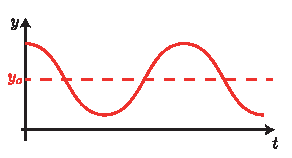
\includegraphics[draft=\pfig]{L2/Fig1_4sol.pdf}
\pincludegraphics{L2/Fig1_4sol_blank.pdf}{L2/Fig1_4sol.pdf}
\p{SHM around the equilibrium point $y_o$.}}

\begin{marginfigure}
\pincludegraphics{L2/Fig1_5_blank.pdf}{L2/Fig1_5.pdf}
\caption{The simple pendulum of mass $m$ and length $L$.} \label{Fig:SimplePendulum}
\end{marginfigure}
\begin{examplebox}{The Simple Pendulum}
Consider the simple pendulum, as shown in Figure \ref{Fig:SimplePendulum}. We model this by assuming that $m$ is a \emph{point mass} connected to the anchor point by a \emph{massless, inextensible string}. 

The path of the mass traces out part of a circle. We will call the arc length along this path $s$. 

Let's also call the tension force in the string $\vec{T}$, which pulls the mass towards the anchor point. 

The restoring force along the arc of the circle is:
\begin{align}
\p{F_r = -mg \sin \phi}
\end{align}

The tangential component of the acceleration is $\frac{d^2 s}{dt^2}$, which lets us write the tangential component of Newton's second law as
\begin{align}
\p{m \frac{d^2 s}{dt^2} = -mg \sin \phi}
\end{align}

For small angles $\sin \phi \simeq s/L$:
\begin{align}
\frac{d^2 s}{dt^2} = \p{- \underbrace{\frac{g}{L}}_{\omega^2} s \qquad \textrm{or} \qquad \frac{d^2 s}{dt^2} + \omega^2 s = 0}
\end{align}
and $s = s_o \cos(\omega t \delta)$ with $\omega = \sqrt{g/L}$. 

Thus for \emph{small displacements}, the period of the pendulum is \emph{independent} of mass of the bob, and depends only on the length of the pendulum. 

Notice that the pendulum \emph{does not} exhibit true SHM for \emph{any} angle. If the angle is less than around $10^\circ$, the motion is close to, and can be \emph{modelled} as, simple harmonic. 
\end{examplebox}

\section{Energy in Simple Harmonic Motion}
\vspace{-0.5cm}
\newthought{We remember from basic mechanics} that for any \emph{conservative} force that there is a direct link to the potential energy of the system, given by \marginnote[0.5cm]{\p{E.g. gravity near the Earth's surface:
\begin{align}
U(x) &= m g x\nonumber\\
F &= mg\nonumber
\end{align}}}
\begin{align}
\p{F_x = - \frac{dU}{dx}}
\end{align}
For SHM we know that $F_x = - kx$, so we can write 
\begin{align}
U(x) &= \int \p{\underbrace{\textcolor{black}{kx}}_{\mathclap{-F_x}}} dx \\
\p{U(x)} &\p{= \frac{1}{2} k x^2}
\end{align}
\marginnote[-2cm]{
\pincludegraphics{L2/Quadratic_potential_blank.pdf}{L2/Quadratic_potential.pdf}
}
This quadratic/parabolic dependence of potential energy on displacement is a \emph{general result} for anything moving with SHM. 

The kinetic energy of the oscillator is given by
\begin{align}
\p{E_{\rm kin} = \frac{1}{2} m v^2}
\end{align}
and the total energy at any moment of time is
\p{
\begin{align}
E_{\rm tot} &= U + E_{\rm kin} \nonumber\\
E_{\rm tot} &= \frac{1}{2} k x^2 + \frac{1}{2}m v^2
\end{align}
}
For any oscillator we can write
\begin{align}
x &= A \cos(\omega t + \delta)\nonumber \\
v &= -A \omega \sin(\omega t + \delta)\nonumber\\
k &= m \omega^2 \nonumber
\end{align}
therefore \marginnote[1cm]{Total Energy of SHM\\ \p{Remembering the trig identity \begin{align}\cos^2(\theta) + \sin^2(\theta) = 1\nonumber\end{align}}}
\begin{align}
E_{\rm tot} &= \frac{1}{2}k A^2 \cos^2(\omega t + \delta) + \frac{1}{2} \p{\underbrace{\textcolor{black}{m \omega^2}}_{k}} A^2 \sin^2(\omega t + \delta) \nonumber\\
&= \p{\frac{1}{2} k A^2}
\end{align}
From this we can conclude that \emph{energy in SHM is conserved}!

\section{The General Applicability of Simple Harmonic Motion}
\vspace{-0.5cm}
\newthought{In SHM, the restoring force} is zero ($F_r = 0$) at the equilibrium point. As $F_r = -\frac{dU}{dx}$, that means the potential energy at this point has either a local maximum or a minimum. 

For \emph{small displacements}, we may expand $U(x)$ in a Taylor Series: \marginnote[-0.5cm]{\p{$f(x) = f(0) + \frac{1}{1!} f'(0)x + \frac{1}{2!} f''(0) x^2 + \frac{1}{3!} f'''(0) x^3 + \ldots$}}
\begin{align}
U(x) = U(0) + x \p{\underbrace{\textcolor{black}{\frac{dU}{dx}(0)}}_{0}} + \frac{1}{2}x^2 \frac{d^2 U}{dx^2}(0) + \ldots
\end{align}

If we chose the zero point of the potential energy such that $U(0) = 0$, then the first two terms of the equation above are equal to zero. Thus we can write that, approximately,  \marginnote[1cm]{Potential Energy for SHM\\
\p{
\begin{align}
U &= \frac{1}{2}k x^2 \nonumber\\
\frac{dU}{dx} &= kx (= -F_x)\nonumber\\
\frac{d^2 U}{dx^2} &= k \nonumber
\end{align}
}}
\marginnote{\p{For the general case:}
\pincludegraphics{L2/General_Quadratic_Potential_blank.pdf}{L2/General_Quadratic_Potential.pdf}}
\begin{align}
\p{U(x) \simeq \frac{1}{2} kx^2}
\end{align}
where $k = \frac{d^2 U}{dx^2}(0)$. 

\noindent \emph{What happens if $k = \frac{d^2 U}{dx^2}(0) < 0$? Clearly the SHM differential equation and solution no longer apply. Is this a stable equilibrium? }

\noindent \emph{Why is the Simple Harmonic Oscillator a good approximation for so many systems we encounter?}

\marginnote{\emph{End of Lecture 2}}




